\documentclass{easychair}

\usepackage{paralist}
\usepackage{xcolor}
\usepackage{amsmath} 
\usepackage{hyperref}
\usepackage{graphicx}
\usepackage{subcaption}
\usepackage{booktabs}
\usepackage{siunitx}
\usepackage{pgfplotstable}
\usepackage{tabularx}
\usepackage{xspace}

\usepackage{tikz}
\usetikzlibrary{arrows,trees,backgrounds,automata,shapes,decorations,plotmarks,fit,calc,positioning,shadows,chains,shapes.geometric}
\tikzstyle{nnedge} = [-{stealth},shorten >=0.1cm, shorten <=0.05cm,line width=0.8pt,black]

\DeclareMathOperator*{\argmax}{arg\,max}
\DeclareMathOperator*{\argmin}{arg\,min}

\newcommand{\relu}{\text{ReLU}\xspace{}}

\newcommand{\sat}{\texttt{SAT}}
\newcommand{\unsat}{\texttt{UNSAT}}

\newtheorem{definition}{Definition}


\sisetup{
  round-mode          = places, 
  round-precision     = 7, 
}
   
\hypersetup{
    colorlinks=true,
    linkcolor=magenta,
    urlcolor=blue,
    breaklinks,
    citecolor=blue
}

\pgfplotstableset{
  multistyler/.style 2 args={
    @multistyler/.style={display columns/##1/.append style={#2}},
    @multistyler/.list={#1}
  }
}


\newcommand{\bracketR}[1]{\left(#1\right)}
\newcommand{\bracketS}[1]{\left(#1\right)}
\newcommand{\bracketC}[1]{\left(#1\right)}
\newcommand{\innerproduct}[1]{\left<#1\right>}
\newcommand\norm[1]{\left\lVert#1\right\rVert}


\newcommand{\guy}[1]{\marginpar{\textcolor{orange}{Guy: #1}}}
\newcommand{\ben}[1]{\marginpar{\textcolor{blue}{Ben: #1}}}

\begin{document}

\title{Minimal Modifications of Deep Neural Networks using Verification}
\author{
Ben Goldberger\inst{1} \and
Yossi Adi\inst{2} \and
Joseph Keshet\inst{2} \and
Guy Katz\inst{1}
}
\institute{
The Hebrew University of Jerusalem, Israel \\
  \{jjgold, guykatz\}@cs.huji.ac.il
  \and
  Bar Ilan University, Israel \\
  yossiadidrum@gmail.com, jkeshet@cs.biu.ac.il
}
\authorrunning{Goldberger, Adi, Keshet and Katz}
\titlerunning{Verifying the Resilience of Neural Network Watermarking}

\maketitle

%% Length: 15 pages

\begin{abstract}
  Deep neural networks (DNNs) are revolutionizing the way complex
  systems are designed, developed and maintained. As part of the life cycle of
  DNN-based systems, there is often a need to modify a DNN in subtle
  ways that affect certain aspects of its behavior, while leaving
  other aspects of its behavior unchanged (e.g., if a bug is discovered and needs to
  be fixed, without altering other functionality). Unfortunately,
  retraining a DNN is often difficult and expensive, and may produce a new
  DNN that is quite different from the original.
  We leverage recent
  advances in DNN verification and propose a technique for modifying
  a DNN according to certain requirements, in a way that is
  \emph{provably minimal}, does not require any retraining, and is
  thus less likely to
  affect other aspects of the DNN's behavior. Using a proof-of-concept
  implementation, we demonstrate the usefulness and potential of
  our approach in addressing two real-world needs: (i) measuring the
  resilience of DNN watermarking schemes; and (ii) bug repair in
  already-trained DNNs.
\end{abstract}

\section{Introduction}
\label{sec:introduction}


\emph{Deep neural networks} (\emph{DNNs}) are quickly becoming the
state of the art in many domains in computer science.  In fields such
as computer vision~\cite{KrSuHi12}, speech
recognition~\cite{HiDeYuDaMoJaSeVaNgSaKi12}, game
playing~\cite{SiHuMaGuSiVaScAnPaLaDi16}, and many others, DNNs have
been repeatedly demonstrating excellent performance, often matching or
even surpassing that of other, hand-crafted solutions.  As a result of
their empiric success, DNNs are changing the way software is being
designed~\cite{GoSoTaCaRiBaAmTeMa18}, and are rapidly being adopted by
users in academia and industry.

The increasing pervasiveness of DNNs is causing a growing need for
modifying already-trained DNNs, as part of their operation and
maintenance. One notable example where this occurs is the
\emph{Machine Learning as a Service} (\emph{MLaaS})
paradigm~\cite{RiGrCa15}, where vendors release almost-fully-trained
DNNs, which clients then fine-tune for their own needs. The motivation
for this paradigm is that training modern DNNs often requires
particular expertise, as well as considerable computing resources,
which clients do not always posses. Another example where modifying an
existing DNN might occur is in \emph{patching}~\cite{SoTh19}: when a
bug is discovered in an existing DNN, a user might wish to modify it
in a way that removes the undesirable behavior, but which leaves
unaffected as many of the DNN's other behaviors as possible. In these
cases, retraining the DNN from scratch might produce a DNN that is
very different from the original, and is thus undesirable; and other
techniques, for modifying an existing DNN, may be used.

These two examples, and others, share the same main characteristics: an
existing DNN needs to be changed in a small way, which removes some
behaviors but keeps others unchanged. Existing approaches for
addressing this need are heuristic-based, and are not guaranteed to
produce the desired results (e.g.,~\cite{KaLe18,KaFu18,SoTh19}).

Here, we propose a novel approach for tackling this challenge, based
on \emph{neural network
  verification}~\cite{HuKwWaWu17,KaBaDiJuKo17Reluplex}. DNN
verification is an emerging field, aimed at proving DNN correctness.
Existing techniques allow users to specify properties that involve the
DNN's inputs and outputs, and then they either prove that these properties hold
or provide a counter-example. Here, we show how to reduce the problem
of making changes to the DNN itself into a DNN verification
problem. Specifically, we propose a method for constructing a new DNN,
and then pose a verification query on that DNN that is satisfiable if
and only if the original DNN can be modified in the desired way. Due
to the soundness of the underlying DNN verification techniques that we
use, our technique affords formal guarantees about the modified DNN
--- specifically, that it is as close as possible to the original, and
that it satisfies the specific constraints.


%We also show how
% our technique can be used to identify minimal changes to DNNs, e.g. in
% the context of correcting their behaviors for certain inputs. The use
% of verification in these contexts guarantees the soundness of our
% approach.


% The MLaaS paradigm holds great potential, but raises two issues that
% must be addressed: \emph{authentication of ownership}, and
% \emph{minimality of changes}.

We demonstrate the applicability of our approach in two domains of interest:

\medskip\noindent
\textbf{Authentication of Ownership.}
As part of the MLaaS paradigm, when vendors allow clients access to an almost-fully-trained network,
they are typically interested in collecting fees and royalties from
each client. This business model compensates the vendor for designing
and training the network, which are not simple tasks. In order to
accomplish this, vendors now seek to imprint their DNNs with
\emph{watermarks} --- secret inputs, known only to the vendors, for which the DNN reacts in
unexpected ways~\cite{AdBaPiKeWatermarking}. The idea is that even if the network is modified by
the client, it will still react unexpectedly to the watermark inputs. This would give vendors a way to
recognize, and then claim ownership, over the networks they had
trained.

DNN watermarking holds promise, but raises a concern: if users are
expected to make modifications to the DNN in order to adjust it to
their needs, could they (accidentally or intentionally) remove the
watermarks? In order to address this concern, we require techniques
for generating \emph{resilient watermarks}, i.e. watermarks that are
difficult to remove without excessively changing the DNN (and
potentially damaging its functionality in the process).

We show how our proposed verification-based technique can be used to
measure the resilience of watermarks within a DNN. Our approach can
thus be used to assess individual DNNs before their release, and also to
to compare and rank different watermarking schemes, according to
the resilience of the watermarks that they produce.

\medskip\noindent \textbf{Minimality of Changes.}
Modifying an already-trained DNN is a complex task, which may be
required under various circumstances --- for example, when
verification shows that a desirable property is violated. 
We show how our approach can be used in order to remove such
violations. Specifically, we propose to maintain a list of points on which
the DNN is known to produce a faulty result, and find a modification
to the DNN that simultaneously corrects the behavior on all of these
points. After each iteration, the network is verified; and if
the property is still violated, meaning that additional faulty inputs
are discovered, these inputs are added to the list of
points, and the process is repeated.

\medskip

For evaluation purposes, we created a proof-of-concept implementation
of our approach as a Python framework. As its underlying DNN
verification backends, our
tool uses the Marabou DNN verification
engine~\cite{KaHuIbJuLaLiShThWuZeDiKoBa19Marabou}, and the Gurobi LP
solver~\cite{gurobi}. We then used our implementation to measure the resilience
of a recently-proposed watermarking
scheme~\cite{AdBaPiKeWatermarking}, and also to correct faulty
behavior of a DNN for an airborne collision avoidance
system~\cite{JuLoBrOwKo16,KaBaDiJuKo17Reluplex}. Our results clearly
indicate the usefulness of our approach to real-world examples.

The rest of this paper is organized as follows. In
Section~\ref{sec:background} we provide the necessary background on
DNNs, DNN watermarking, and DNN verification. Next, in
Section~\ref{sec:verifyWatermarks} we introduce our technique for
casting the minimal DNN modification problem into a DNN verification
problem. In Section~\ref{sec:applications} we describe how to apply 
our technique in the context of watermark resilience and DNN patching.
Section~\ref{sec:evaluation} describes our implementation and
evaluation of the approach.
We discuss related work in Section~\ref{sec:relatedWork},
and conclude in Section~\ref{sec:conclusion}.

\section{Background}
\label{sec:background}

\subsection{Neural Networks}
A deep neural network is comprised of an input layer, an output layer,
and multiple hidden layers in between. Each layer consists of multiple
nodes (also called neurons), each of which is connected to nodes from
the preceding layer. Each edge that connects two neurons is assigned a
predetermined weight. An example appears in
Fig.~\ref{fig:dnnExample}. Weight selection
is performed during the DNN's training phase, which is beyond our
scope here --- see, e.g.,~\cite{FoBeCu16}. 


\begin{figure}[htp]
\centering
\scalebox{0.7}{
\def\layersep{2.5cm}
\begin{tikzpicture}[shorten >=1pt,->,draw=black!50, node distance=\layersep]
    \tikzstyle{every pin edge}=[<-,shorten <=1pt]
    \tikzstyle{neuron}=[circle,fill=black!25,minimum size=17pt,inner sep=0pt]
    \tikzstyle{neuron node}=[neuron, fill=blue!50];
    \tikzstyle{annot} = [text width=4em, text centered]

    % Draw the input layer nodes
    \foreach \name / \y in {1,...,4}
        \node[neuron node, pin=left:Input \#\y] (I-\name) at (0,-\y) {};

    % Draw the hidden layer a nodes
    \foreach \name / \y in {1,...,5}
        \path[yshift=0.5cm]
            node[neuron node] (Ha-\name) at (\layersep,-\y) {};
	
	% Draw the hidden layer b nodes
    \foreach \name / \y in {1,...,5}
        \path[yshift=0.5cm]
            node[neuron node] (Hb-\name) at (2*\layersep,-\y) {};

	% Draw the output layer nodes
    \foreach \name / \y in {1,...,3}
        \path[yshift=-0.5cm]
        	node[neuron node, pin={[pin edge={->}]right:Output \#\y}] (O-\name) at (3*\layersep,-\y) {};    
    % Connect every node in the input layer with every node in the
    % hidden layer.
    \foreach \source in {1,...,4}
        \foreach \dest in {1,...,5}
            \draw[nnedge] (I-\source) -- (Ha-\dest);

    % Connect every node in the hidden layer a with the hidden layer b
    \foreach \source in {1,...,5}
        \foreach \dest in {1,...,5}
            \draw[nnedge] (Ha-\source) -- (Hb-\dest);
	% Connect every node in the hidden layer b with the output layer
    \foreach \source in {1,...,5}
        \foreach \dest in {1,...,3}
            \draw[nnedge] (Hb-\source) -- (O-\dest);

    % Annotate the layers
    \node[annot,above of=Ha-1, node distance=1cm] (hla) {Hidden layer \#1};
    \node[annot,above of=Hb-1, node distance=1cm] (hlb) {Hidden layer \#2};
    \node[annot,left of=hla] {Input layer};
    \node[annot,right of=hlb] {Output layer};
\end{tikzpicture}
}
\caption{An example of a simple deep neural network. The network has
  an input layer of size $4$, two hidden layers of size $5$ each, and an
  output layer of size $3$. The edge weights are omitted.}
\label{fig:dnnExample}
\end{figure}

The neural network is evaluated by assigning values to the input
nodes, and then iteratively propagating these values through the
network, computing the values of additional layers one at a
time. Eventually, the values of the output layer are computed, and
these constitute the network's output.  The value of each hidden node
in the network is computed by calculating a weighted sum of node
values from the preceding layer, and then applying a non-linear
\emph{activation function}~\cite{FoBeCu16}.  For simplicity, we focus
here on the Rectified Linear Unit (ReLU) activation
function~\cite{NaHi10}, although our technique is directly applicable
to additional functions as well.  When the ReLU activation function,
$\relu{}(x) = \max{}(0, x)$, is applied to a node, its value is
computed as the maximum between $0$ and the weighted sum computed
according to the values of nodes from
the previous layer.

More formally, let $N$ denote a DNN. We
denote the number of layers in $N$ by $n$, and use $s_i$ to denote the
dimension of layer $i$ (i.e., the number of neurons that it contains).
Layer $1$ is the input layer, layer $n$ is the output layer, and
layers $2,\ldots,n-1$ are the hidden layers.
We use $v_{i,j}$  to denote the value of the $j$'th node of layer $i$,
and use $V_i$ to denote the column vector $[v_{i,1},\ldots,v_{i,s_i}]^T$.
When evaluating $N$ we are given $V_1$, and need to compute $V_n$.
This computation is 
performed by using the predefined weights and biases to compute the
layer assignments one by one, each time applying the activation
functions (ReLUs, in our case) to each node. Each layer $2\leq i\leq
n$
is associated
with a 
weight matrix $W_i$ of size $s_{i}\times s_{i-1}$, and also a bias vector $B_i$ of size
$s_i$. The entry of $W_i$ at the $j$'th row and $k$'th column, denoted
$W_i[j,k]$, represents the weight assigned to the edge from
neuron $v_{i-1,k}$ to neuron $v_{i,j}$.
Each hidden layer ($2\leq i \leq n-1$) 
is computed as
\[
V_i = \relu{}(W_i  V_{i-1} + B_i),
\]
with the ReLU
function being applied element-wise.
This rule is applied repeatedly for each layer until $V_{n-1}$ is
calculated.
The final, output layer is
computed similarly, but without an activation function:
\[
  V_n = W_n  V_{n-1} + B_n
\]
For simplicity, in the rest of the paper we assume that
the bias vector $B_i$ is always $0$.

DNNs are often used as \emph{classifiers}, assigning to each input a
label from a finite set of possible labels $L=\{l_1,\ldots,l_{s_n}\}$. In this case, each neuron
in the output layer corresponds to one possible label, and the label
whose neuron is assigned the highest value is the label to which the
input is classified. Thus, an input $V_1$ is classified to label $l_i$
if and only if $v_{n,i}>v_{n,j}$ for every $j\neq i$ (draws are
resolved arbitrarily). We sometimes use the alternative phrasing,
\[
  N(V_1) = \argmax_{1\leq i\leq s_n}\{v_{n,i}\}
\]
A small, running example appears in Fig.~\ref{fig:toyExample}. Our
example has $3$ layers, each of size $2$. The weights are depicted
over the edges (all biases are assumed to be 0). For a given input
$V_1=\langle 3, 4 \rangle$ the second layer assignment is computed as
\[
  V_2=\langle \relu{}(1\cdot 3-2\cdot 4),\relu{}(2\cdot 3-1\cdot
  4)\rangle = \langle 0,2 \rangle
 \]
 and the output layer is computed as
 \[
   V_3= \langle 1 \cdot 0 -1 \cdot 2, -1 \cdot 0 +1  \cdot 2\rangle =
   \langle -2, 2 \rangle
 \]
 Observe that, by definition, the \relu{} activation functions are not applied to the
 output layer. This implies that input $\langle 3, 4\rangle$ is
 classified to label $2$, because $v_{3,2}> v_{3,1}$.

\begin{figure}[htp]
  \begin{center}
    \scalebox{1} {
      \def\layersep{3cm}
    \begin{tikzpicture}[shorten >=1pt,->,draw=black!50, node distance=\layersep,font=\footnotesize]
    \tikzstyle{neuron}=[circle,fill=black!25,minimum size=17pt,inner sep=0pt]
    \tikzstyle{neuron node}=[neuron, fill=blue!50];
    \tikzstyle{annot} = [text width=4em, text centered]

      \node[neuron node] (I-1) at (0,-1 cm) {$v_{1,1}$};
      \node[neuron node] (I-2) at (0,-2 cm) {$v_{1,2}$};

      \path[yshift=0.5cm]
      node[neuron node] (H-1) at (\layersep,-1) {$v_{2,1}$};
      \path[yshift=-0.5cm]
      node[neuron node] (H-2) at (\layersep,-2) {$v_{2,2}$};

      \node[neuron node] at (2*\layersep, -1) (O-1) {$v_{3,1}$};
      \node[neuron node] at (2*\layersep, -2) (O-2) {$v_{3,2}$};

      % Connect every node in the hidden layer with the output layer

      \draw[nnedge] (I-1) -- node[above] {$1$} (H-1);
      \draw[nnedge] (I-1) -- node[below] {$2$} (H-2);
      \draw[nnedge] (I-2) -- node[above] {$-2$} (H-1);
      \draw[nnedge] (I-2) -- node[below] {$-1$} (H-2);
      \draw[nnedge] (H-1) -- node[above] {$1$} (O-1);
      \draw[nnedge] (H-1) -- node[above] {$-1$} (O-2);
      \draw[nnedge] (H-2) -- node[below] {$-1$} (O-1);
      \draw[nnedge] (H-2) -- node[below] {$1$} (O-2);
      
      % Annotate the layers
      \node[annot,above of=H-1, node distance=1cm] (l) {$V_2$};
      \node[annot,left of=l] {$V_1$};
      \node[annot,right of=l] {$V_3$};
    \end{tikzpicture}
    }
	\caption{A small neural network.}
    \label{fig:toyExample}
  \end{center}
\end{figure}

\subsection{Neural Network Verification}


Let $N$ denote a neural network, and let $P,Q$ denote predicates
that encode some constraints over the DNN's inputs and outputs, respectively.
\emph{DNN verification}~\cite{HuKwWaWu17,KaBaDiJuKo17Reluplex} is a field that seeks to answer the question:
does there exist an input $x$ to the DNN such that $P(x)$ and
$Q(N(x))$ both hold, where $N(x)$ represents the network's output when
evaluated on input $x$. Typically, $P$ encodes a set of inputs of
interest, whereas $Q$ encodes the \emph{negation} of a desired
property. If the verification query is \unsat{}, i.e. no such input
$x$ exists, then the desired property is said to hold. Otherwise, the
verification tool returns a concrete counter-example $x_0$ for which
the property in question is violated.


Recently there have been multiple tools and approaches suggested for
solving the DNN verification problem: these include Satisfiabiltiy
Modulo Theories (SMT) based
techniques~\cite{KaBaDiJuKo17Reluplex,KaHuIbJuLaLiShThWuZeDiKoBa19Marabou},
approaches based on mixed integer linear
programming~\cite{Ehlers2017,TjXiTe19}, abstract interpretation based
techniques~\cite{GeMiDrTsChVe18}, and several others
(e.g.,~\cite{HuKwWaWu17,NaKaRySaWa17}). The problem is known to be
difficult, and has been shown to be NP-complete even when restricted
to simple cases~\cite{KaBaDiJuKo17Reluplex} (networks with
piecewise-linear activation functions, and properties $P$ and $Q$ that
are conjunctions of linear constraints). Consequently, most existing approaches
have limited scalability, and are highly sensitive to DNN size.


\section{Minimal DNN Modification as a Verification Problem}
\label{sec:verifyWatermarks}

\subsection{Modifying DNNs}

In all DNN verification approaches to date (to the best of our
knowledge), the goal is to verify a fixed DNN. In other words, $N$ is
given, and a particular input $x_0$ is sought that satisfies certain constraints.
The novelty of our approach is in changing this definition, fixing
the input point $x_0$ (or multiple inputs) and searching for a
\emph{different DNN} $N$ such that certain conditions hold.
More formally, we define the problem as follows:

\begin{definition}\textbf{The DNN Modification Problem.}
  Let $N$ denote a DNN, let $X$ denote a set of fixed input points
  $X=\{x_1, \ldots, x_n\}$, and let $Q$ denote a predicate over the
  classifications $N(x_1),\ldots,N(x_n)$ of the points of $X$. The
  \emph{DNN modification problem} is to find a new DNN, $N'$, such that
  $Q(N'(x_1),\ldots,N'(x_n))$ holds, and such that the distance
  between $N$ and $N'$ is at most some $\delta>0$.
\end{definition}

In this definition we did not yet specify how to measure the distance
between $N$ and $N'$. Multiple measures of distance could be used, but for the
motivating problems that we consider (e.g., verifying the resilience
of watermarks, or finding minimal fixes for erroneous inputs), it
makes sense to require that $N$ and $N'$ share the same topology, and
to define the distance between $N$ and $N'$ according to the
difference in these network's weights. We note that a DNN modification
is trivial if the property $Q$ holds for the original network $N$,
i.e. if $Q(N(x_1),\ldots,N(x_n))$ holds; in that case, $N$ itself is a
feasible solution to the modification problem.

\begin{definition}\textbf{DNN Distance.}
  Let $N^1$ and $N^2$ denote two DNNs with identical topology,
  i.e. the same number of layers ($n^1=n^2$), and the same number of
  neurons in every pair of matching layers ($s_i^1=s_i^2$ for all
  $1\leq i \leq n^1$). We define the $L$-distance between $N^1$ and $N^2$,
  denoted $\norm{N^1-N^2}_L$, as:
  \[
    \norm{N^1-N^2}_L =    \bracketsR{\sum_{i=2}^{n^1}\sum_{j=1}^{s_{i}^1}\sum_{k=1}^{s_{i-1}^1}
    \abs{W^1_i[j,k] - W^2_i[j,k]}^L}^{1/L}
  \]
\end{definition}

Intuitively, this definition of distance compares the weight matrices
of the two networks, element-wise; it computes the $L$-distance
between each two corresponding edge weights as the $L$-norm of the differnce between two vectors.

Fig.~\ref{fig:toyExampleModified} shows how these definitions are applied
to our toy example from Fig.~\ref{fig:toyExample}. Network $N^2$ is
obtained from the original network, $N^1$, by slightly modifying its
edge weights but maintain the same layer structue. The distance
between these DNNs is:
\guy{Ben: does this definition even work for $L_\infty$? Maybe we should
  write that we we treat all weights as a long vector, and compute the
  norm of the vector of differences}

\begin{align*}
	&\norm{N^1-N^2}_L=(\bracketsR{\abs{-0.5}^L+\abs{1}^L+\abs{1}^L+\abs{-0.5}^l+\abs{0.5}^L+\abs{0.5}^L)}^{1/L}\\
	&\norm{N^1-N^2}_1=(\abs{-0.5}+\abs{1}+\abs{1}+\abs{-0.5}+\abs{0.5}+\abs{0.5}+0+0)=4\\
	&\norm{N^1-N^2}_\infty=max\bracketsC{\abs{-0.5},\abs{1},\abs{1},\abs{-0.5},\abs{0.5},\abs{0.5},0,0}=1
\end{align*}

\begin{figure}[htp]
  \begin{subfigure}{0.5\linewidth}
      \def\layersep{3cm}
    \begin{tikzpicture}[shorten >=1pt,->,draw=black!50, node distance=\layersep,font=\footnotesize]
    \tikzstyle{neuron}=[circle,fill=black!25,minimum size=17pt,inner sep=0pt]
    \tikzstyle{neuron node}=[neuron, fill=blue!50];
    \tikzstyle{annot} = [text width=4em, text centered]

      \node[neuron node] (I-1) at (0,-1 cm) {$v^1_{1,1}$};
      \node[neuron node] (I-2) at (0,-2 cm) {$v^1_{1,2}$};

      \path[yshift=0.5cm]
      node[neuron node] (H-1) at (\layersep,-1) {$v^1_{2,1}$};
      \path[yshift=-0.5cm]
      node[neuron node] (H-2) at (\layersep,-2) {$v^1_{2,2}$};

      \node[neuron node] at (2*\layersep, -1) (O-1) {$v^1_{3,1}$};
      \node[neuron node] at (2*\layersep, -2) (O-2) {$v^1_{3,2}$};

      % Connect every node in the hidden layer with the output layer
      \draw[nnedge] (I-1) -- node[above] {$1$} (H-1);
      \draw[nnedge] (I-1) -- node[below] {$2$} (H-2);
      \draw[nnedge] (I-2) -- node[above] {$-2$} (H-1);
      \draw[nnedge] (I-2) -- node[below] {$-1$} (H-2);
      \draw[nnedge] (H-1) -- node[above] {$1$} (O-1);
      \draw[nnedge] (H-1) -- node[above] {$-1$} (O-2);
      \draw[nnedge] (H-2) -- node[below] {$-1$} (O-1);
      \draw[nnedge] (H-2) -- node[below] {$1$} (O-2);

    \end{tikzpicture}
    \caption{$N^1$}
  \end{subfigure}
  \begin{subfigure}{0.5\linewidth}
      \def\layersep{3cm}
    \begin{tikzpicture}[shorten >=1pt,->,draw=black!50, node distance=\layersep,font=\footnotesize]
    \tikzstyle{neuron}=[circle,fill=black!25,minimum size=17pt,inner sep=0pt]
    \tikzstyle{neuron node}=[neuron, fill=blue!50];
    \tikzstyle{annot} = [text width=4em, text centered]

      \node[neuron node] (I-1) at (0,-1 cm) {$v^2_{1,1}$};
      \node[neuron node] (I-2) at (0,-2 cm) {$v^2_{1,2}$};

      \path[yshift=0.5cm]
      node[neuron node] (H-1) at (\layersep,-1) {$v^2_{2,1}$};
      \path[yshift=-0.5cm]
      node[neuron node] (H-2) at (\layersep,-2) {$v^2_{2,2}$};

      \node[neuron node] at (2*\layersep, -1) (O-1) {$v^2_{3,1}$};
      \node[neuron node] at (2*\layersep, -2) (O-2) {$v^2_{3,2}$};

      % Connect every node in the hidden layer with the output layer
      \draw[nnedge] (I-1) -- node[above] {$1.5$} (H-1);
      \draw[nnedge] (I-1) -- node[below] {$1$} (H-2);
      \draw[nnedge] (I-2) -- node[above] {$-3$} (H-1);
      \draw[nnedge] (I-2) -- node[below] {$-0.5$} (H-2);
      \draw[nnedge] (H-1) -- node[above] {$0.5$} (O-1);
      \draw[nnedge] (H-1) -- node[above] {$-1.5$} (O-2);
      \draw[nnedge] (H-2) -- node[below] {$-1$} (O-1);
      \draw[nnedge] (H-2) -- node[below] {$1$} (O-2);
      
    \end{tikzpicture}
    \caption{$N^2$}
  \end{subfigure}
  \caption{The DNN from Fig.~\ref{fig:toyExample}, denoted $N^1$, and
    a modified version thereof, denoted $N^2$.}
  \label{fig:toyExampleModified}
\end{figure}

Finally, we will typically be interested in finding $N'$ that is
closest to $N$. This is formalized as follows:
\begin{definition}\textbf{The DNN Minimal Modification Problem.}
  Let $N$ denote a DNN, let $X$ denote a set of fixed input points
  $X=\{x_1, \ldots, x_n\}$, and let $Q$ denote a predicate over the
  classifications $N(x_1),\ldots,N(x_n)$ of the points of $X$. The
  \emph{DNN minimal modification problem} is to find a new DNN $N'$
  that solves the DNN modification problem (for $N, X$ and $Q$), such that for every other
  $N''$ that solves the modificaiton problem it holds that
  $\norm{N'-N}\leq \norm{N''-N}$.
\end{definition}
We observe that given a decision procedure for solving the modification
problem, solving the minimal modification problem can be performed by
repeatedly invoking that procedure as part of a binary search.

\subsection{Minimal Modifications as DNN Verification}

A straightforward approach for solving the minimal DNN modification
problem is to cast it as an optimization problem, and use an
off-the-shelf optimization tool. Specifically, the goal would be to
minimize $\norm{N^1-N^2}_p$, while maintaining the constraint
\guy{Ben, where did underscore p come from?}
$Q(N'(x_1),\ldots, N'(x_n))$. Unfortunately, such an optimization
problem is highly non-convex and high-dimensional, and is hence very
difficult to solve.

We illustrate this issue in Fig.~\ref{fig:optimizeAllLayers}, again using
our running example from~\ref{fig:toyExample}. In the modified network
depicted in the figure, $N'$, we keep the original
weights of the DNN, but to each edge also add a variable,
$w_1,\ldots,w_8$. In order to solve the minimization problem, we would
need to minimize the $w_i$ variables (the exact expression to be minimized
depends on the distance metric in use), but we would also need to
ensure that the predicate $Q$ holds for $N'$, and this would involve
solving non-convex, high-degree constraints.

For example, suppose $X=\{\langle 3, 4\rangle\}$, and that $Q(\langle
3,4\rangle)=v_{3,1}\geq v_{3,2}$. Recall that the original network
classified $\langle 3,4\rangle$ as label 2, and so our goal here is to
modify the network so that it classifies this point as label 1.
The expressions for $v_{3,1}$ and $v_{3,2}$ are:
\begin{align*}
  v_{3,1}&=
  (1+w_5)\cdot  \relu{}(3(1+w_1)+4(-2+w_3))
  +
  (-1+w_7)\cdot \relu{}(3(2+w_2)+4(-1+w_4))
  \\
  v_{3,2}&=
  (-1+w_6)\cdot \relu{}(3(1+w_1)+4(-2+w_3))
  +
  (1+w_8) \cdot \relu{}(3(2+w_2)+4(-1+w_4))
\end{align*}
For larger networks, these constraints would become significantly more complex.

\begin{figure}[htp]
\begin{center}
	  \def\layersep{3cm}
      \def\layersepb{1cm}
    \begin{tikzpicture}[shorten >=1pt,->,draw=black!50, node distance=\layersep,font=\footnotesize]
    \tikzstyle{neuron}=[circle,fill=black!25,minimum size=17pt,inner sep=0pt]
    \tikzstyle{neuron node}=[neuron, fill=blue!50];
    \tikzstyle{annot} = [text width=4em, text centered]

      \node[neuron node] (I-1) at (0,-1 cm) {$v_{1,1}$};
      \node[neuron node] (I-2) at (0,-2 cm) {$v_{1,2}$};

      \path[yshift=0.5cm]
      node[neuron node] (H-1) at (\layersep,-1) {$v_{2,1}$};
      \path[yshift=-0.5cm]
      node[neuron node] (H-2) at (\layersep,-2) {$v_{2,2}$};

      \node[neuron node] at (2*\layersep, -1) (O-1) {$v_{3,1}$};
      \node[neuron node] at (2*\layersep, -2) (O-2) {$v_{3,2}$};

      % Connect every node in the hidden layer with the output layer
      \draw[nnedge] (I-1) -- node[above,rotate=10] {$1+w_1$} (H-1);
      \draw[nnedge] (I-1) -- node[below,rotate=-25] {$2+w_2$} (H-2);
      \draw[nnedge] (I-2) -- node[above,rotate=25] {$-2+w_3$} (H-1);
      \draw[nnedge] (I-2) -- node[below,rotate=-10] {$-1+w_4$} (H-2);
      \draw[nnedge] (H-1) -- node[above,rotate=-10] {$1+w_5$} (O-1);
      \draw[nnedge] (H-1) -- node[above,rotate=-25] {$-1+w_6$} (O-2);
      \draw[nnedge] (H-2) -- node[below,rotate=25] {$-1+w_7$} (O-1);
      \draw[nnedge] (H-2) -- node[below,rotate=10] {$1+w_8$} (O-2);
      
      % Annotate the layers
      \node[annot,above of=H-1, node distance=1cm] (l) {$V_2$};
      \node[annot,left of=l] {$V_1$};
      \node[annot,right of=l] {$V_3$};
    \end{tikzpicture}	
	\caption{The DNN from Fig.~\ref{fig:toyExample}, with
          modifications to its edges expressed as variables $w_1,\ldots,w_8$.}
    \label{fig:optimizeAllLayers}
    \end{center}
\end{figure}


In order to mitigate this issue and render the DNN modification problem easier to
solve for large networks, we focus on a restricted version of
the problem in which the changes in weights are
limited to a \emph{single layer}. We argue that under this
restriction, the DNN modification problem reduces into standard DNN
verification problem. The intuition is as follows: let $N$ be a DNN,
and let $W_i$ (for some fixed $i$, $2\leq i\leq n$) be the only weight matrix of $N$ that
we wish to modify. Observe some fixed input point $x\in X$, and let
$V_{i-1}$ denote the evaluation of layer $i-1$ for this $x$. In the
modified network $N'$, layers $1,\ldots,i-1$ will be assigned the same
values as in $N$, i.e, $V_k=V'_k$ for all $1\leq k\leq i-1$. The
changes in assignment begin only in layer $i$, where it holds that
\[
  V_i' = \relu{}(W_i'V'_{i-1}) = \relu{}((W_i+W_\epsilon)V'_{i-1})
\]
where $W_\epsilon$ represents the change in weights. We note that
$W_i$ and $V'_{i-1}$ are fixed; the only variables here are the
entries of $W_\epsilon$. This means that we can construct a new DNN,
denoted $\bar{N}$, whose input neurons are the values of $W_\epsilon$,
followed by a layer that computes $\relu{}((W_i+W_\epsilon)V'_{i-1})$,
and then feeds into layers $i+1,\ldots,n$ of the original network.

%% Guy got here

We again illustrate this using our running example --- see
Fig.~\ref{fig:changeJustOneLayer}. The variable arethe entries of $W_\epsilon=[w_1,w_2,w_3,w_4]$ and the output of the network for input $V_1=(3,4)$ is:
\\
\begin{math}
v_{3,1}=1\cdot\relu{}((1+w_1)\cdot 3+(-2+w_3)\cdot 4)+(-1)\cdot\relu{}((2+w_2)\cdot 3+(-1+w_4)\cdot 4)\\
v_{3,2}=(-1)\cdot\relu{}((1+w_1)\cdot 3+(-2+w_3)\cdot 4)+1\cdot\relu{}((2+w_2)\cdot 3+(-1+w_4)\cdot 4)
\end{math}

And for the $\norm{W_\epsilon}_1$ and $\norm{W_\epsilon}_\infty$ the constraint and the optimization problem are piecewise-linear. 

\begin{figure}[htp]
\begin{center}
	  \def\layersep{3cm}
      \def\layersepb{1cm}
    \begin{tikzpicture}[shorten >=1pt,->,draw=black!50, node distance=\layersep,font=\footnotesize]
    \tikzstyle{neuron}=[circle,fill=black!25,minimum size=17pt,inner sep=0pt]
    \tikzstyle{neuron node}=[neuron, fill=blue!50];
    \tikzstyle{annot} = [text width=4em, text centered]

      \node[neuron node] (I-1) at (0,-1 cm) {$v_{1,1}$};
      \node[neuron node] (I-2) at (0,-2 cm) {$v_{1,2}$};

      \path[yshift=0.5cm]
      node[neuron node] (H-1) at (\layersep,-1) {$v_{2,1}$};
      \path[yshift=-0.5cm]
      node[neuron node] (H-2) at (\layersep,-2) {$v_{2,2}$};

      \node[neuron node] at (2*\layersep, -1) (O-1) {$v_{3,1}$};
      \node[neuron node] at (2*\layersep, -2) (O-2) {$v_{3,2}$};

      % Connect every node in the hidden layer with the output layer
      \path (I-1) edge[] node[above,rotate=10] {$1+w_1$} (H-1);
      \path (I-1) edge[] node[below,rotate=-25] {$2+w_2$} (H-2);
      \path (I-2) edge[] node[above,rotate=25] {$-2+w_3$} (H-1);
      \path (I-2) edge[] node[below,rotate=-10] {$-1+w_4$} (H-2);
      \path (H-1) edge[] node[above,rotate=-10] {$1$} (O-1);
      \path (H-1) edge[] node[above,rotate=-25] {$-1$} (O-2);
      \path (H-2) edge[] node[below,rotate=25] {$-1$} (O-1);
      \path (H-2) edge[] node[below,rotate=10] {$1$} (O-2);
      
      % Annotate the layers
      \node[annot,above of=H-1, node distance=1cm] (l) {$V_2$};
      \node[annot,left of=l] {$V_1$};
      \node[annot,right of=l] {$V_3$};
    \end{tikzpicture}
	\caption{ }
    \label{fig:changeJustOneLayer}
    \end{center}
\end{figure}

In the previous example, we reduced the DNN modification problem into
the DNN verification problem for a set $X$ that contained a
\emph{single point}. The reduction when $X$ contains multiple points
is similar; we simply duplicate the DNN that we construct $n$ times, creating a
copy for each $x\in X$. This allows us to solve the problem
simultaneously for the multiple points. However, because DNN
verification is NP-complete in the size of the DNN being
verified~\cite{KaBaDiJuKo17Reluplex}, this renders the problem
significantly more difficult to solve. In
Section~\ref{sec:outputLayer} we discuss a method for
simplifying the process in some cases.

Finally, we note that the restricted version of the problem, in which
we only allow changing a single layer of network, is interesting in
its own right. Specifically, it is is sufficiently expressive for...
\guy{TODO: justify why this is interesting}


\subsection{Private Case: Modifying the DNN's Output Layer}
\label{sec:outputLayer}

Even when the DNN modification problem is limited to changes in a
single layer of the DNN, the existence of many points in the set $X$
can render the resulting DNN verification problem difficult to
solve. However,  we observe if the changes are limited to the \emph{output
  layer} of the DNN, the resulting problem is typically easier to
solve. Intuitively, the reason is that if only this layer is changed,
the resulting DNN verification problem contains a smaller number of
neurons than when an earlier layer is changed.

In addition, if the distance metric in use is the $L_\infty$ norm,
changing only the output layer renders the resulting DNN verification
problem \emph{completely linear}. This means that it can then be solved using
linear programming solvers, which tend to scale much better than DNN
verification tools.

\begin{figure}[htp]
\begin{center}
	  \def\layersep{3cm}
      \def\layersepb{1cm}
    \begin{tikzpicture}[shorten >=1pt,->,draw=black!50, node distance=\layersep,font=\footnotesize]
    \tikzstyle{neuron}=[circle,fill=black!25,minimum size=17pt,inner sep=0pt]
    \tikzstyle{neuron node}=[neuron, fill=blue!50];
    \tikzstyle{annot} = [text width=4em, text centered]

      \node[neuron node] (I-1) at (0,-1 cm) {$v_{1,1}$};
      \node[neuron node] (I-2) at (0,-2 cm) {$v_{1,2}$};

      \path[yshift=0.5cm]
      node[neuron node] (H-1) at (\layersep,-1) {$v_{2,1}$};
      \path[yshift=-0.5cm]
      node[neuron node] (H-2) at (\layersep,-2) {$v_{2,2}$};

      \node[neuron node] at (2*\layersep, -1) (O-1) {$v_{3,1}$};
      \node[neuron node] at (2*\layersep, -2) (O-2) {$v_{3,2}$};

      % Connect every node in the hidden layer with the output layer
      \path (I-1) edge[] node[above,rotate=10] {$1$} (H-1);
      \path (I-1) edge[] node[below,rotate=-25] {$2$} (H-2);
      \path (I-2) edge[] node[above,rotate=25] {$-2$} (H-1);
      \path (I-2) edge[] node[below,rotate=-10] {$-1$} (H-2);
      \path (H-1) edge[] node[above,rotate=-10] {$1+w_1$} (O-1);
      \path (H-1) edge[] node[above,rotate=-25] {$-1+w_2$} (O-2);
      \path (H-2) edge[] node[below,rotate=25] {$-1+w_3$} (O-1);
      \path (H-2) edge[] node[below,rotate=10] {$1+w_4$} (O-2);
      
      % Annotate the layers
      \node[annot,above of=H-1, node distance=1cm] (l) {$V_2$};
      \node[annot,left of=l] {$V_1$};
      \node[annot,right of=l] {$V_3$};
    \end{tikzpicture}
	\caption{ }
    \label{fig:changeLastLayer}
    \end{center}
\end{figure}

We demonstrate with our running example \ref{fig:changeLastLayer}:
Suppose we're unhappy with the network. The original network output was $V_3=(-2,2)$ so our constraint over the output is $v_{3,2}\leq v_{3,1}$
We're only changing weights in the last layer so the network is fixed until the last layer. We calculate $V_2=(0,2)$ and define a LP problem for minimizing the $L_\infty$ norm of the change.

\begin{align*}
Minimize:\quad & M \\
Subject\ to:\quad & -M \leq w_1\leq M \\
& -M \leq w_2\leq M \\
& -M \leq w_3\leq M \\
& -M \leq w_4\leq M \\
& v_{3,1}=(1+w_1)\cdot 0+(-1+w_3)\cdot 2 \\
& v_{3,2}=(-1+w_2)\cdot 0+(1+w_4)\cdot 2 \\
& v_{3,2}\leq v_{3,1}
\end{align*}

A feasible solution to this LP is $w_3=1$ and $w_1,w_2,w_4=0$


\section{Applications}
\label{sec:applications}

\subsection{Watermark Resilience}
As briefly discussed in Section~\ref{sec:introduction}, there is now a
growing need to imprint DNNs with \emph{watermarks}: secret inputs,
known to the creator of the DNN, on which the DNN produces unexpected
outputs. Watermarks are important for the MLaaS business model, where
a vendor sells a mostly-trained DNN to clients, who then fine-tune
it for their own needs. The key requirement is that even if the
network undergoes some changes, the watermark input will still produce
the original, unexpected output, allowing the vendor to recognize the
DNN.

More formally, given a DNN $N$, a watermark is just an input point $x$
with a specific label $l$. Typically, a network will have a finite set of
watermarks $X$. Creating this set of watermarks is done at time of
training --- see, e.g.,~\cite{AdBaPiKeWatermarking} for details. We
say that a set $X=\{x_1,\ldots,x_n\}$ of watermarks is $\delta$-resilient if for every
DNN $N'$ such that $\norm{N-N'}\leq \delta$, it holds that
$N(x_i)=N'(x_i)$ for all $1\leq i \leq n$. Clearly, a watermarking
scheme that produces watermarks that are more resilient is preferable.

Solving the DNN minimal modification problem can thus serve two
purposes in the context of watermarking:
\begin{inparaenum}[(i)]
  \item given a specific DNN $N$ and a set $X$ of watermarks, it can
    measure the resilience of $X$ (i.e., the maximal amount of changes
    the network can withstand without ``forgetting'' the watermarks);
    and
  \item given multiple schemes for watermarking DNNs, i.e. for
    producing the set $X$, it can compare the effectiveness of the
    schemes by checking the resilience of the resulting watermarks
    (on some set of DNNs).
\end{inparaenum}
  
\subsection{Minimal Repair}
Despite their overall excellent performance, DNN-based systems are as
prone to error as any other system. Specifically, many erroneous
behaviors have been observed in various DNNs, e.g. for image
recognition~\cite{EyEvFeLiRaXiPrKo18,SzZaSuBrErGoFe13} and for airborne collision
avoidance~\cite{JuLoBrOwKo16,KaBaDiJuKo17Reluplex}. Once such a bug is
discovered, it is not immediately clear how to correct it. One
approach would be to retrain the network, but this may be expensive
or impossible for some clients. The approach that we propose here is
simply to identify a \emph{minimal} change to the DNN that removes the
undesirable behavior. We argue that it is useful to focus on a minimal
change here, as such a change is less likely to change the behavior of
the network for other inputs, on which its behavior is currently acceptable.

Finding minimal repairs for a DNN $N$ can be cast into our
formulation, as follows. Given a set of erroneous points
$X=\{x_1,\ldots,x_n\}$ and their set of \emph{correct} labels
$l_1,\ldots,l_n$, we seek a new DNN $N'$ such that $N'(x_i)=l_i$ for
all $1\leq i \leq n$, and such that 
 $\norm{N-N'}$ is minimal. 

\section{Evaluation}
\label{sec:evaluation}

\subsection{Watermark Removal}

In order to apply our approach to measure the resilience of
watermarked networks, we trained a watermarked DNN over the MNIST
digit recognition dataset~\cite{mnist}. The DNN was of a modest size:
it had an input layer with 784 nodes, a single hidden layer with $150$
nodes, and final output layer with $10$ nodes. The input and output layers were fully
connected, and the hidden layer had the \relu{} activation function
applied to its nodes. We used the
method proposed in~\cite{AdBaPiKeWatermarking} to create a set
$X=\{x_1,\ldots, x_{100}\}$ of $100$ watermarks, each assigned a label
$N(x_i)$; an example appears in Fig.~\ref{fig:inputExample}.
\guy{TODO: fix broken ref, subfigure is messing it up}

\begin{figure}[htp]
  \centering
  \begin{subfigure}{0.4\linewidth}
    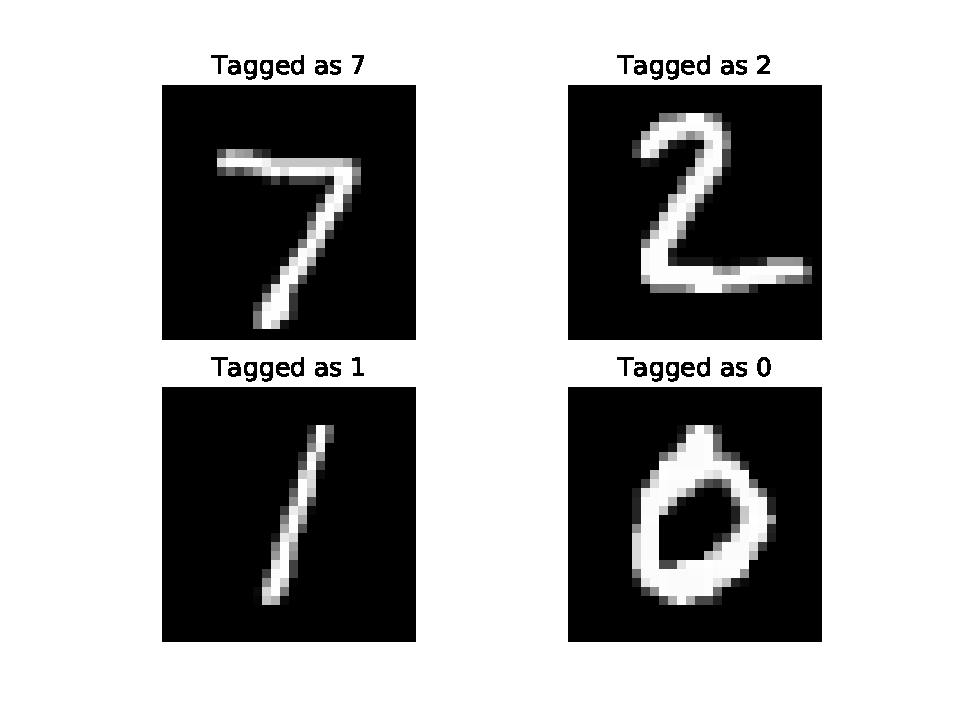
\includegraphics[width=\linewidth]{../data/mnist.pdf}
    \caption{Standard MNIST inputs.}
  \label{fig:mnistExample}
  \end{subfigure}
  \begin{subfigure}{0.4\linewidth}
    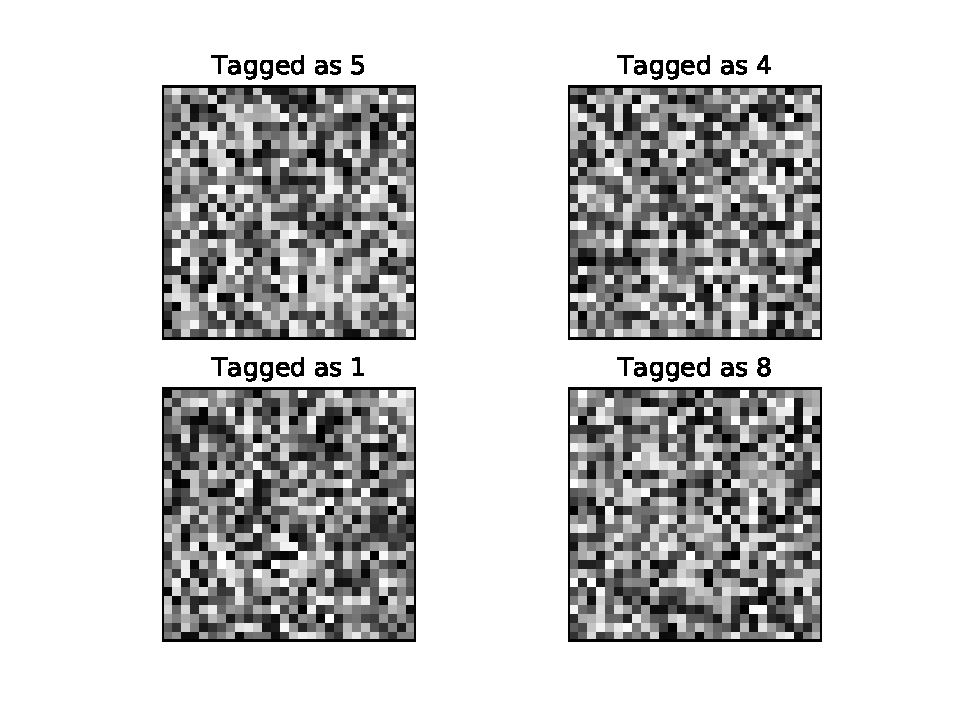
\includegraphics[width=\linewidth]{../data/wm.pdf}
     \caption{Watermark inputs.}
  \label{fig:noiseExample}
  \end{subfigure}
  \caption{Inputs to our MNIST digit-recognition DNN. The inputs of the
  left are standard, and are correctly classified by the network. The
  inputs on the right are the watermarks: the network was trained in a
  specialized way to make it assign those particular labels to those inputs.}
\label{fig:inputExample}
\end{figure}

Next, we ran a series of experiments to identify modifications to the
network that would remove some, or all, of these watermarks. For
simplicity, we
focused on changes to the network's last layer. As a measure of
distance, we used the $L_1$ and $L_\infty$ norms, which are popular
distance metrics in the ML community and are supported my many DNN
verification tools.

\medskip\noindent \textbf{Removing a Single Watermark.}
We began by measuring the minimal change to the network required to
remove each individual watermark. More specifically, for each
watermark $x\in X$ we found the closest network $N'$ such that
$N(x)\neq N'(x)$. We note that we did not explicitly specify $N'(x)$,
i.e. did not require that $N'$ classify $x$ in a particular way; we
only required that the new label be different than the original. We
ran the experiment once with $L_1$, and once with $L_\infty$; the
results are depicted in Fig.~\ref{fig:minSingle}.


\begin{figure}[htp]
  \centering
  \begin{subfigure}{0.4\linewidth}
    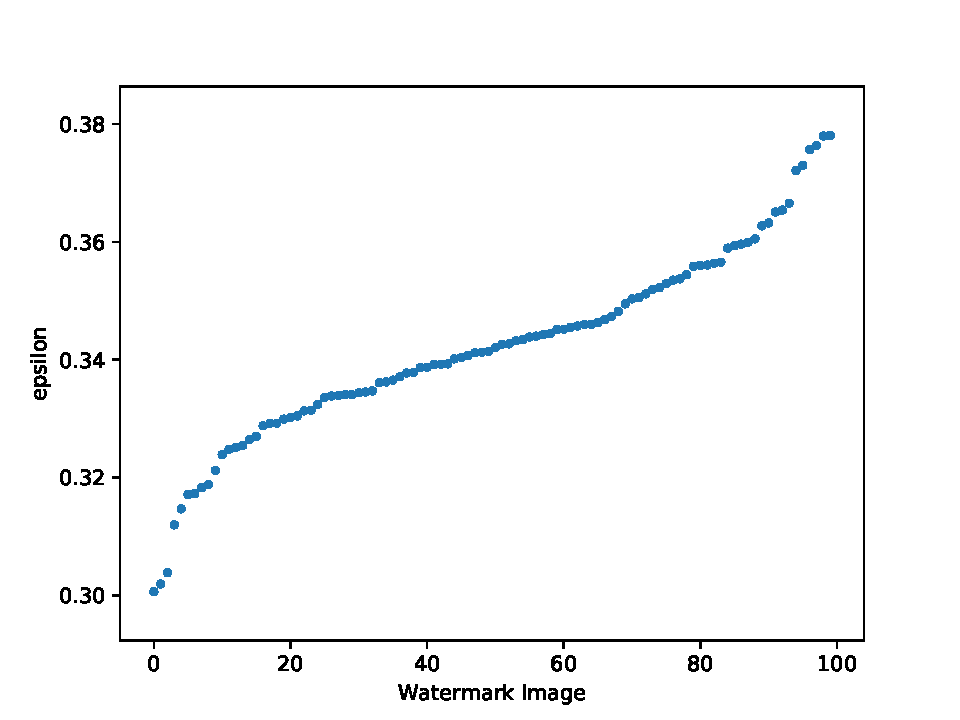
\includegraphics[width=\linewidth]{../data/results/problem3/mnist_w_wm_sorted.pdf}
     \caption{The Minimal $\norm{\varepsilon}_{\infty}$ for every watermark image}
  	\label{fig:minSingleLP}
  \end{subfigure}
  \begin{subfigure}{0.4\linewidth}
    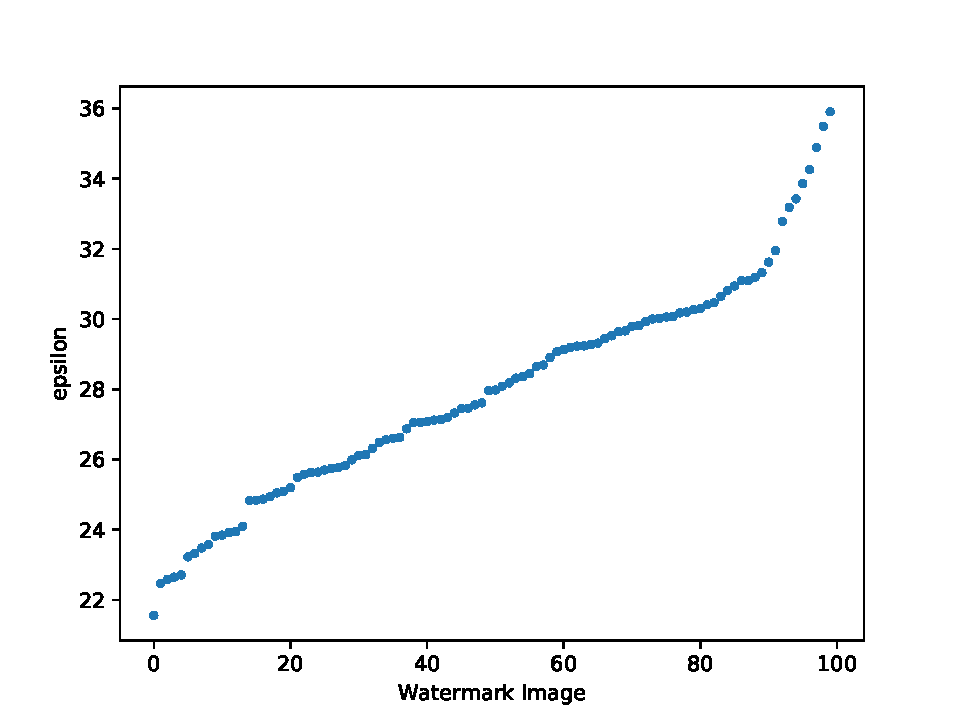
\includegraphics[width=\linewidth]{../data/results/problem2/mnist_w_wm_sorted.pdf}
    \caption{The Minimal $\norm{\varepsilon}_1$ for every watermark image}
  	\label{fig:minSingleNotLP}
  \end{subfigure}
%  \caption{Notice the scale of the graphs, the $\ell_\infty$ values are much smaller then the $\ell_1$ values. As expected}
\label{fig:minSingle}
\end{figure}

Analyzing these results exposes several interesting properties of the
watermark inputs. For example, we observed 
that for every single watermark $x$, the minimatance network that
was found classified $x$ as the second-highest label assigned to
it by the original network. This result indicates
that a resilient watermark should have a
significant gap between the score assigned to its actual label and
the score of its second-highest label. We also observed that some
watermarks are \emph{significantly} more difficult to remove than
others; specifically, in the $L_\infty$ case, the more resilient
watermarks were approximately $26\%$ more difficult to remove than
others, and in the $L_1$ case --- about $70\%$ more
difficult. \guy{TODO: ben, please check these numbers with the raw
  data. Also, can you check if the hardest benchmarks had larger gaps
  between the winner and runner-up label?}
This indicates a very wide range of watermark resilience, and can
serve as a measure for the DNN's trainer to assess the watermark effectiveness.

The experiment also exposes some of the differences between the two
distance metrics used, i.e. $L_1$ and $L_\infty$. Not surprisingly,
the distances in the $L_1$ case are generally larger than those in the
$L_\infty$ case: this is because the $L_\infty$ norm allows us to
change multiple edges ``at no additional cost'', and thus effect the
network's outcome more effectively; whereas $L_1$ distance counts
every edge weight that changes. In
Fig.~\ref{fig:lastLayerExampleSingle} we visualize this on one
of the watermarks; we see that indeed, when using the $L_\infty$ norm,
almost all the edges were touched, whereas the $L_1$ norm caused the
change to occur only in a single edge.

 
\begin{figure}
\centering
  \begin{subfigure}{0.4\linewidth}
  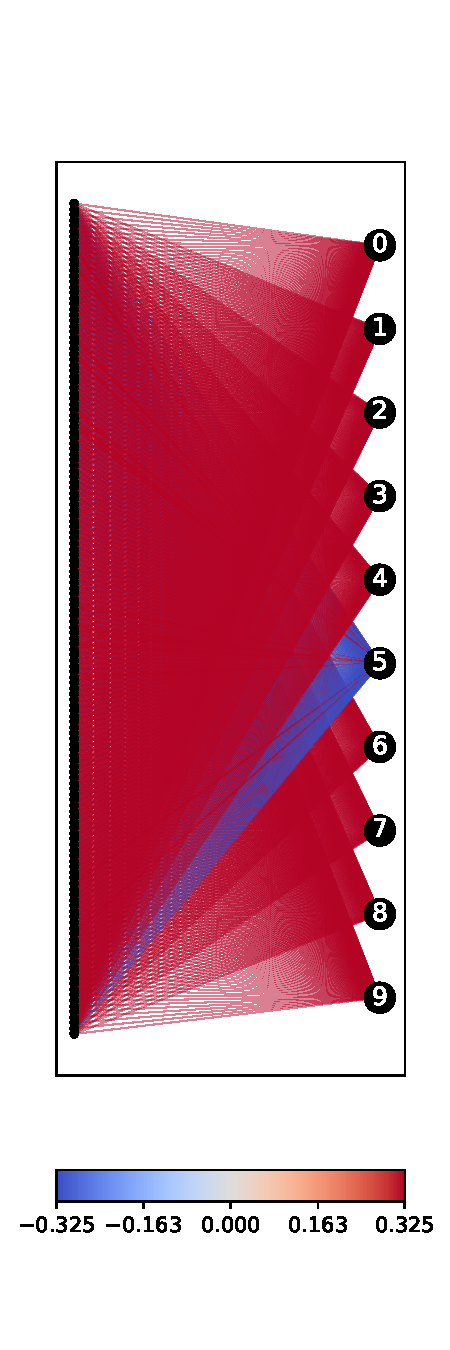
\includegraphics[width=\linewidth]{../data/results/problem3/last_layer_1_wm_example.pdf}
     \caption{The Minimal change according to $\ell_\infty$ for a single input}
  \end{subfigure}
  \begin{subfigure}{0.4\linewidth}
    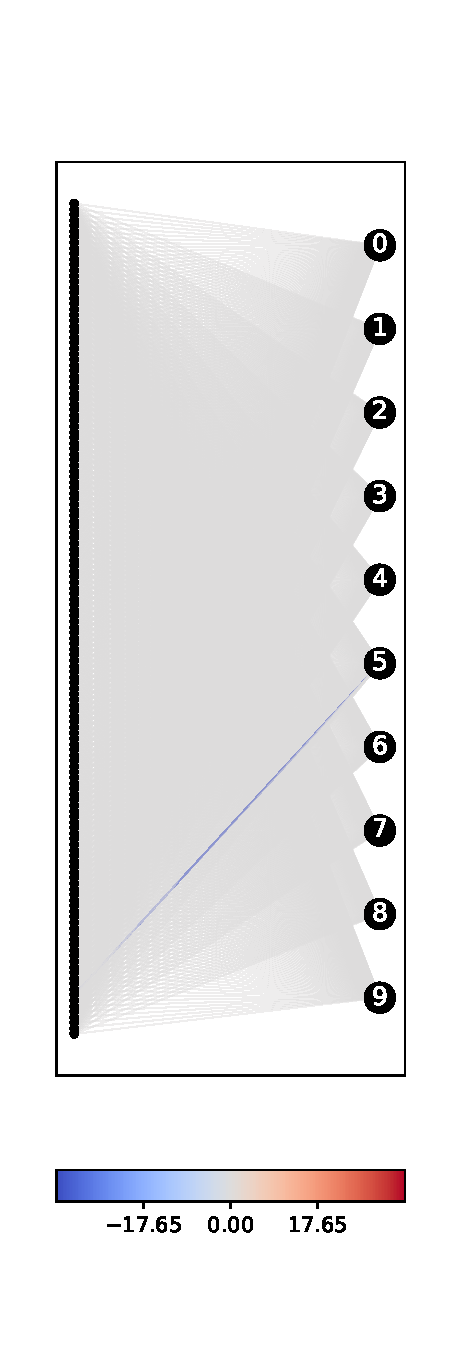
\includegraphics[width=\linewidth]{../data/results/problem2/last_layer_1_wm_example.pdf}
    \caption{The Minimal change according to $\ell_1$ for a single input}
  \end{subfigure}
  \caption{Examples of the change to the last layer. Positive change is colored red and negative change is colored blue. There are $150$ nodes on the left.}
  \label{fig:lastLayerExampleSingle}
\end{figure}


In addition, we were also interested to see the effect of removing a
watermark on the network's overall accuracy --- as it is likely to
assume that a user seeking to remove watermarks will also attempt to
maintain the network's original performance. After removing each
benchmark, we used the MNIST dataset to result the accuracy of the
modified network and compared it to the original. As it turns out, the
results (depicted in Table~\ref{table:singleWatermark})
vary widely between $L_1$ and $L_\infty$. We observe that using 
$L_1$ gives better accuracy result on average, but can lead to poor
accuracy in extreme cases; whereas the $L_\infty$ norm leads to a much
more consistent result (there minimal accuracy and the maximal
accuracy are quite close), although the average accuracy is lower than
that of $L_1$. 

\begin{table}
\resizebox{\textwidth}{!}{
	\pgfplotstabletypeset[
	every head row/.style={before row=\hline,after row=\hline\hline},
	every last row/.style={after row=\hline},
	col sep=comma,
	columns/Norm/.style={string type},
	every column/.style={column type/.add={|}{}},
	every last column/.style={column type/.add={}{|}}
	]{../data/results/mnist_w_wm_1_wm.csv}
	}
\caption{Minimal changes and Accuracy}
\label{table:singleWatermark}
\end{table}

\medskip\noindent \textbf{Removing Multiple Watermarks.}
Next, we addressed the issue of modifying our DNN in a way that
removes multiple watermarks, simultaneously. Specifically, we wanted
to change the weights of the DNN's output layer in a way that caused
the misclassification of an arbitrary number of watermarks.

As discussed in Section~\ref{sec:outputLayer}, the problem of modifying the network's
output layer when using the $L_\infty$ norm is significantly easier
than other variants; and indeed, using Gurobi as our backend
verification tool we were able to find modifications
that remove as many as all of the watermarks. In the $L_1$ case,
performance became an issue, and so we focused on removing as many as
5 watermarks simultaneously. The results are depicted in
Table~\ref{table:multipleWatermarks}. We see that a few benchmarks can
still be removed while maintaining a reasonable level of accuracy; but
that, at least in the $L_\infty$ case, removing all watermarks renders
the network quite useless. We thus conclude that using $100$
watermarks is sufficient for this particular network.


\begin{table}
\begin{subtable}{1\textwidth}
\centering
\resizebox{\linewidth}{!}{
	\pgfplotstabletypeset[
	every head row/.style={before row=\hline,after row=\hline\hline},
	every last row/.style={after row=\hline},
	col sep=comma,
	columns/Norm/.style={string type},
	every column/.style={column type/.add={|}{}},
	every last column/.style={column type/.add={}{|}}
	]{../data/results/problem3/mnist_w_wm_summary.csv}
	}
\caption{Change and accuracy when solving for minimal $L_\infty$ change.}
\end{subtable}
\begin{subtable}{1\textwidth}
\centering
\resizebox{\linewidth}{!}{
	\pgfplotstabletypeset[
	every head row/.style={before row=\hline,after row=\hline\hline},
	every last row/.style={after row=\hline},
	col sep=comma,
	columns/Norm/.style={string type},
	every column/.style={column type/.add={|}{}},
	every last column/.style={column type/.add={}{|}}
	]{../data/results/problem4/mnist_w_wm_summary.csv}
	}
\caption{Change and accuracy when solving for minimal $L_1$ change.}
\end{subtable}
\caption{Minimal changes and accuracy degradation when simultaneously removing multiple watermarks.}
\label{table:multipleWatermarks}
\end{table}


\subsection{Removing Undesirable Behavior}

In a separate experiment, we evaluated the effectiveness of our
approach in correcting undesirable behaviors in a real-world DNN that
is part of the ACAS Xu system for Airborne Collision
Avoidance~\cite{JuLoBrOwKo16}. This airborne system, which is part of new
standard, is currently being developed by the FAA. It is intended to
read sensor information regarding other nearby aircraft, and produce a
horizontal turning advisory in order to avoid a possible collision
with these aircraft. One possible implementation of the system that is
being considered includes a family of 45 DNNs~\cite{JuLoBrOwKo16}.

For our experiment, we focused on one of the ACAS Xu DNNs in which a
bug has been discovered using formal
verification~\cite{KaBaDiJuKo17Reluplex}; specifically, it has been
observed that for a specific input, the network advises a strong turn
where it should advise a weak turn or no turn at all. We used our
technique to seek a minimal modification to the DNN in question that
would correct this behavior. Because our goal was to make the property
hold, and not necessarily correct a single faulty input to the DNN, we
applied the following loop:

\begin{enumerate}
\item Use verification to check whether property $\varphi$ holds.
\item If not, add the counter-example to $S$.
\item Find a minimal modification of $N$ that corrects the behavior
  for  all points currently in $S$.
\end{enumerate}

This process terminates either when the property holds, or when a
timeout value is reached. 

For our ACAS Xu experiment, we observed that the property in question
still did not hold after the first iteration, i.e. after fixing the
first counter-example. We fixed a second counter-example, and then
timed-out while attempting to fix the third counter-example.
The results are depicted in Fig.~\ref{fig:lastLayerACASXU}.

\begin{figure}
\centering
\begin{subfigure}{0.2\linewidth}
  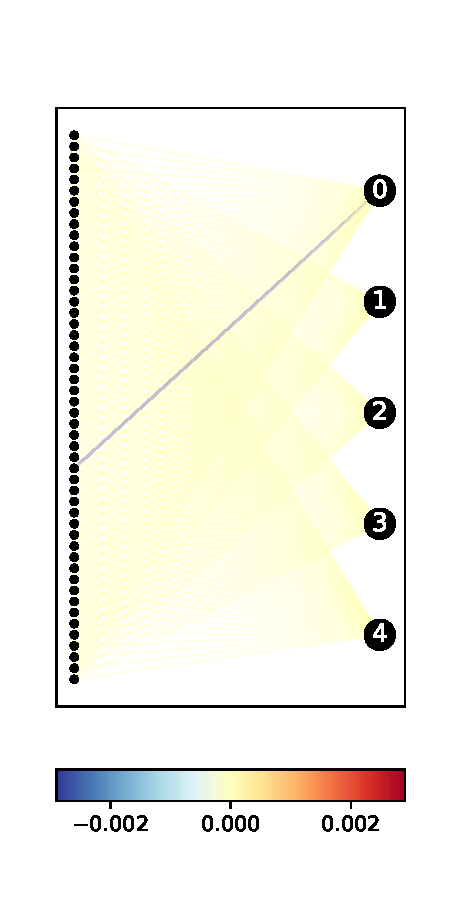
\includegraphics[width=\linewidth]{./images/ACASXU_2_9_1_vals.pdf}
  \caption{First iteration inputs change}
\end{subfigure}
\begin{subfigure}{0.2\linewidth}
  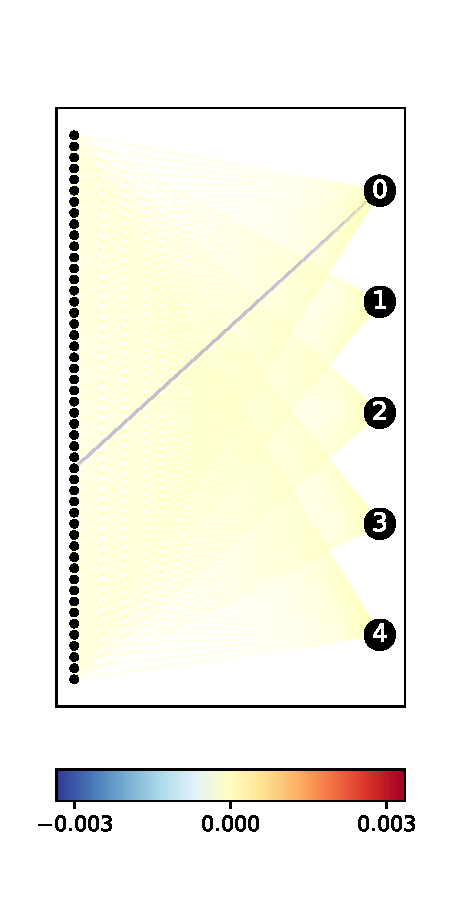
\includegraphics[width=\linewidth]{./images/ACASXU_2_9_3_vals.pdf}
  \caption{Second iteration inputs change}
\end{subfigure}
\begin{subfigure}{0.2\linewidth}
  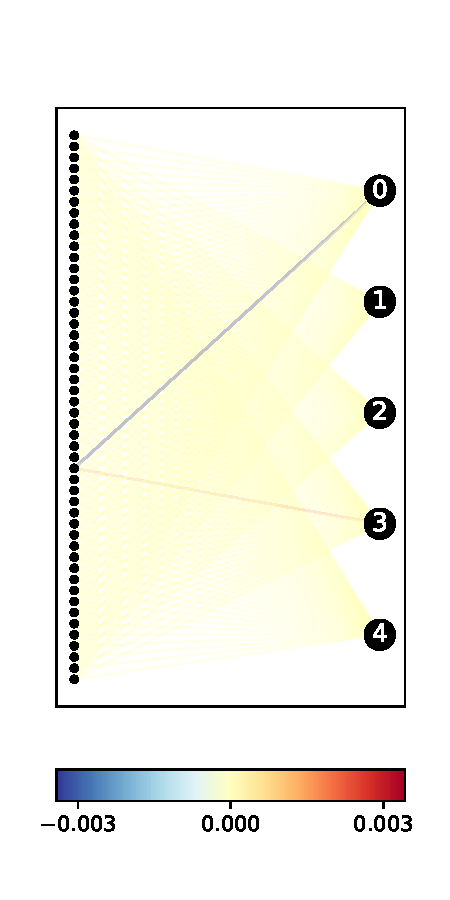
\includegraphics[width=\linewidth]{./images/ACASXU_2_9_all1_vals.pdf}
  \caption{Third iteration inputs change}
\end{subfigure}
\caption{Change to the last layer for one of the ACAS Xu networks.}
\label{fig:lastLayerACASXU}
\end{figure}


\guy{Questions about ACAS Xu: what norm did we use? Are the two graphs
  identical? Was a single edge changed in both?}

\section{Related Work}
\label{sec:relatedWork}

Correcting DNNs in order to remove undesirable behaviors is a general
topic of interest in the ML community. One line of
work~\cite{KaLe18,KaFu18} suggests to augment a malfunctioning DNN
with decision trees that determine when a patch should be
applied. Another line of work~\cite{SoTh19} corrects DNNs using an
iterative encoding of the problem into a sequence of Max-SMT
instances. A key feature of our verification-based approach that
separates it from prior work is that it provides provides formal
guarantees about the minimality of the discovered changes to the DNN
in question.

DNN verification is an emerging field, with many recently-proposed
tools and approaches. These include the use of SMT
solving~\cite{HuKwWaWu17,KaBaDiJuKo17Reluplex,KaHuIbJuLaLiShThWuZeDiKoBa19Marabou},
LP and MILP solving~\cite{Ehlers2017,TjXiTe19}, symbolic interval
propagation~\cite{WaPeWhYaJa18}, abstract
interpretation~\cite{GeMiDrTsChVe18}, and many others
(e.g.,~\cite{BuTuToKoMu18,DuJhSaTi18,LoMa17,NaKaRySaWa17,SiGePuVe19}).
Our technique reduces the DNN minimal modification problem into a DNN
verification problem, and can use many of the aforementioned tools and
techniques as a backend.

DNN watermarking is a general approach for marking DNNs that are to undergo
changes, for which multiple methods have been proposed in recent years~\cite{AdBaPiKeWatermarking,ChRoKo18,LePeTr19,UcNaSaSa17,VeUsTaOcGa11}
Our technique can be applied in order to assess the
performance of watermarking approaches and compare them to each other.


\section{Conclusion and Future Work}
\label{sec:conclusion}

With the fast spreading use of DNNs, there is an increasing need to
make small modifications to already-trained networks --- e.g., as part
of the MLaaS paradigm, or in order to correct erroneous DNN behavior. By
harnessing recent advances in DNN verification, we proposed here a
method for finding the minimal changes required to make a DNN satisfy
certain properties. This technique holds great potential
for users who wish to change a DNN, and also for vendors who
wish to ensure that their DNNs maintain some behavior even if
modified. We demonstrated the applicability of our approach for 
watermark removal, and also for bug correction.

In the future we plan to extend our technique so that it can be
applied when the changes to a DNN occur in more than one layer. In
order to overcome the highly non-linear and non-convex nature of the
problem, we plan to apply compositional techniques: i.e., to break the DNN
down into smaller DNNs, so that the changes to each smaller DNN will only occur in
a single layer. We will then apply our technique to each smaller DNN
separately, and use the results to draw conclusions regarding changes
to the original DNN as a whole. In addition, we plan to research additional
use cases, beyond watermark removal and bug removal, where our technique
could prove useful.

\subsection*{Acknowledgments}
The project was partially supported by grants from the Binational Science
Foundation (2017662) and the Israel Science Foundation (683/18).

\guy{TODO: Ask the Yossis for additional acks}

\bibliographystyle{abbrv}
\bibliography{watermarks}

\end{document}


%%%
%%%% Old text, mostly subsumed and divided into other sections,
%%%% keeping it here for reference
%%%
% We denote the prediction of the original network as 
% \[
%    	d_x := argmax_{i\in \bracketsS{m}}\bracketsC{y_i}
% \]
% And the changed network prediction:
% \[
%    	d'_x := argmax_{i\in \bracketsS{m}}\bracketsC{y'_i}
% \]
% And we seek a change $\varepsilon$ to the last layer so that the prediction changes, i.e. $d_x\neq d'_x$.

% As previously mentioned, we seek a minimal $\varepsilon$ for which the
% label of $x$ changes. As a measure of minimality, we adopt two norms
% that are commonly used in the DNN community: the $L_\infty$ and $L_1$
% norms. Specifically, 
% \begin{equation}
% \label{eq:normInf}
%    		\norm{\varepsilon}_{\infty}=max_{i,j}\bracketsC{\abs{\varepsilon_{i,j}}}
% \end{equation}
% And
% \begin{equation}
% \label{eq:normOne}
%    		\norm{\varepsilon}_1=\sum_{i,j}\abs{\varepsilon_{i,j}}.
% \end{equation}

% When the $\ell_\infty$ norm (\ref{eq:normInf}) is in use, the
% aforementioned requirements give rise to a linear programming
% minimization problem''
% \begin{align*}
% \label{eq:LP}
%     Minimize:\quad & M \\
%     Subject\ to:\quad & \forall i,j\quad -M \leq\varepsilon_{i,j}\leq M \\
%     & y'=(L+\varepsilon)v \\
%     & y'_{d_x} \leq y'_{d'_x} \\
% \end{align*}

% Where the variables are the entries in $\varepsilon,y'$ and $M$.
% For the $\ell_1$ norm (\ref{eq:normOne}), the minimization problem becomes:
% \begin{eqnarray*}
% \label{eq:NotLP}
%     Minimize:\quad & M \\
%     Subject\ to:\quad & \forall i,j\quad -M \leq\sum_{i,j}\abs{\varepsilon_{i,j}}\leq M \\
%     & y'=(L+\varepsilon)v \\
%     & y'_{d_x} \leq y'_{d'_x} \\
% \end{eqnarray*}

% Where the variables are the entries in $\varepsilon,y'$ and $M$.

        
% \subsection{Defining the problem for multiple inputs}
% \label{sec:defineProblem2}

% Our definition to a single input minimal change $\varepsilon$ to the network last layer $L$ can be extended to more then one input very easily by adding more constraint to the problem.
% \\
% Given inputs $\bracketsC{x_1,\cdots,x_k}$ and their respective values:
% \begin{align*}
% \bracketsC{v_1,\cdots,v_k}\quad: & \text{Inputs to the last layer} \\
% \bracketsC{d_1,\cdots,d_k}\quad: & \text{Decisions} \\
% \intertext{Such that}
% \forall 1\leq j\leq k\quad & d_j = argmax_{i\in\bracketsS{m}}\bracketsC{\bracketsR{L v_j}_i}
% \intertext{With chosen new desired decisions
% $\bracketsC{d'_1,\cdots,d'_k}$ Such that}
% \forall 1\leq j\leq k\quad & d'_j \neq d_j
% \end{align*}
% \\
% our minimization problem for the $\ell_\infty$ norm looks like this:
% \begin{equation}
% \label{eq:LPmany}
% \begin{split}
%     Minimize:\quad & M \\
%     Subject\ to:\quad & \forall i,j\quad -M \leq\varepsilon_{i,j}\leq M\\
%     & \forall j\quad y'_j=(L+\varepsilon)v_j \\
%     & \forall j\quad \bracketsR{y'_j}_{d_j} \leq \bracketsR{y'_j}_{d'_j}\\
% 	\intertext{Variables are the entries in $\varepsilon,y'_1,\cdots,y'_k$ and $M$}
% \end{split}
% \end{equation}
% Similarly for the $\ell_1$ norm the minimization problem looks like that:
% \begin{equation}
% \label{eq:NotLPmany}
% \begin{split}
%     Minimize:\quad & M \\
%     Subject\ to:\quad & \forall i,j\quad -M \leq\sum_{i,j}\abs{\varepsilon_{i,j}}\leq M\\
%     & \forall j\quad y'_j=(L+\varepsilon)v_j \\
%     & \forall j\quad \bracketsR{y'_j}_{d_j} \leq \bracketsR{y'_j}_{d'_j}\\
% 	\intertext{Variables are the entries in $\varepsilon,y'_1,\cdots,y'_k$ and $M$}
% \end{split}
% \end{equation}


% As seen in the previous section we have in our hands a minimization problem. One minimization is according to $\ell_\infty$ norm and the other is according to $\ell_a$ norm. In this section we'll show how to convert different problems to the type of minimization problem that was described in the previous section \ref{sec:minimizationProblem}
% For the $\ell_\infty$ norm when choosing new predictions all the constraint of the minimization problems (\ref{eq:LP}) (\ref{eq:LPmany}) are linear. There for we choose to solve the $\ell_\infty$ problem using a linear programming solver.
% On the other hand $\ell_1$ norm minimization problems (\ref{eq:NotLP}) (\ref{eq:NotLPmany}) have non linear constraint so a linear programming solver is not enough. Instead we used a solver that is capable of dealing with piecewise-linear constraints. 

% \subsection{Removing watermarks from neural networks}
% \label{sec:removeWatermarks}
% A watermarked neural network is a neural network that was trained with a set of inputs and their desired outputs such that the network will still function properly on the task it meant to do, and the output of the network on the set of inputs is as desired (The desired output can be irrelevant to the network task). We'll call the set of inputs and outputs the watermarks of the network \cite{AdBaPiKeWatermarking}. These trained networks are called ``Backdoored'' networks \cite{GuDoSi17BadNet}.
% Given a trained watermarked network $N$ with a set of $K$ watermarks inputs and outputs $\bracketsC{\bracketsR{x_1,y_1},\cdots,\bracketsR{x_K,y_K}}$, if we want to remove a specific watermark from the network we can define one of the minimization problems that was described in the previous section (\ref{eq:LP}) (\ref{eq:NotLP}) and search which of the possible decisions (Beside the original decision of the watermark) gives the minimal change.
% When removing a set of watermarks of a size $K$ we defined those minimization problem (\ref{eq:LPmany}) (\ref{eq:NotLPmany}), when solving for multiple watermarks we didn't check with combination of possible decisions gets the minimal change because the number of combinations of possible decisions is exponential in $K$, so in order to save time we used a simple heuristic to decide which combination of decisions to check for. 



%%% Local Variables:
%%% mode: latex
%%% TeX-master: t
%%% End:
